% Working thesis draft: introduction and Chapters 1-4.
% Starting draft for editing - not a final thesis document.
% Preamble follows thesis_outline.tex; report class so chapters number.
% TODO: switch to the university's thesis class once it is chosen.
\documentclass[11pt,a4paper]{report}

\usepackage[margin=1in]{geometry}
\usepackage{setspace}
\usepackage{booktabs}
\usepackage{tabularx}
\usepackage{array}
\usepackage{tikz}
\usetikzlibrary{arrows.meta}
\usepackage{hyperref}
\usepackage[numbers]{natbib}

% Visible marker for missing references, data, and decisions.
\newcommand{\todo}[1]{\textbf{[TODO: #1]}}

\onehalfspacing
\title{Cheap Multi-Robot Autonomous Fleets for Disaster Recovery:\\
Phone-as-Brain Rovers with Depth Sensing, Obstacle Avoidance, and Fleet Command Interfaces}
\author{Yojan Gautam}
\date{\today}

\begin{document}
\maketitle
\tableofcontents

% Introduction. First draft.
% Sources: "Project ARGOS - One Operator Many Robots" deck (Oct 23, 2026),
% thesis_outline.tex, papers_research_questions.md, docs/ARGOS_CURRENT_SUMMARY.md.
% Status claims match the platform repositories as of Oct 23, 2026. No results are reported here.
% Unnumbered so the following background chapter is Chapter 1.
% TODO: if the department numbers the introduction as Chapter 1, drop the star and the addcontentsline.

\chapter*{Introduction}
\addcontentsline{toc}{chapter}{Introduction}
\label{ch:introduction}

\section*{Robots in real missions}

Robots have been part of disaster response for more than two decades, and the same problems keep returning.
At the World Trade Center in 2001, every robot on the pile was teleoperated.
The one robot that was lost and not recovered was a wireless unit: it lost its control link and had no onboard intelligence to move and reacquire the signal~\citep{murphy2004rescue}.
At Fukushima Daiichi in 2011, the concrete walls of the reactor buildings were expected to block radio, so the Quince robot was driven over a cable, and teleoperation had to be simple enough for first responders rather than the researchers who built it~\citep{nagatani2011fukushima}.
At the DARPA Subterranean Challenge Final in 2021, each team was allowed a single Human Supervisor to interact with its robots, and one operator managed eleven robots in the Louisville Mega Cavern~\citep{darpa2021subt,ackerman2021subtoperators}.
At the Champlain Towers South collapse in Surfside, Florida, the same year, drones flew 304 missions for mapping and strategic operations alone, and the drone teams coordinated through a WhatsApp group chat~\citep{murphy2021surfside}.

Read together, these deployments show three recurring failures.
Communication fails, and a robot that depends entirely on its link stops being useful the moment the link drops.
One person ends up juggling several robots with no shared picture of where they are and what they need.
The robots carry too little autonomy for the job, or an amount chosen by trial and error rather than by measurement.
SubT showed that one-person supervision of a fleet is possible.
It also showed its limits: the operator who ran eleven robots described them as ``quite a lot to be managed by a single human operator under a constrained time limit,'' and operators across teams were still the bottleneck for confirming finds, retasking robots, and freeing stuck ones~\citep{ackerman2021subtoperators}.

\section*{One operator, many robots}

This thesis studies the setting those missions point toward: one human operator supervising a fleet of ground robots.
Three questions make that setting hard.

\begin{enumerate}
\item \textbf{Autonomy.} What is the minimum level of autonomy each robot needs to complete a mission, and when should the human step in?
\item \textbf{Attention.} When several vehicles need the operator at the same time, how should the operator's attention be scheduled across them?
\item \textbf{Bandwidth.} How much telemetry can each robot send as the fleet grows, and what should the operator see continuously versus on demand?
\end{enumerate}

These questions interact.
More onboard autonomy means each robot asks for help less often and can survive a lost link, which frees operator attention and reduces the bandwidth each robot needs.
More autonomy also costs development effort, compute on the vehicle, and operator trust, and a robot that is more autonomous than the mission needs is harder to understand when it misbehaves.
The practical goal is the lowest level of autonomy that finishes the job and survives a lost link, with a human takeover always one action away.

\section*{Levels of autonomy}

To make the autonomy question measurable, this thesis uses a six-level ladder for a single ground vehicle (Table~\ref{tab:intro-levels}).
Each level adds one responsibility to the robot and removes one from the human.

\begin{table}[ht]
\centering
\caption{Autonomy levels used in this thesis. Runtime names are the values the ARGOS operator application publishes to Terra.}
\label{tab:intro-levels}
\begin{tabularx}{\textwidth}{@{}l l X l@{}}
\toprule
Level & Name & Robot does & Runtime name \\
\midrule
L0 & Full teleoperation & Nothing on its own; the human controls all motion. & \texttt{teleop} \\
L1 & Assisted teleoperation & The human drives; the rover prevents collisions. & \texttt{assisted\_teleop} \\
L2 & Waypoint, no avoidance & Drives from A to B along predefined waypoints. & \texttt{waypoint\_direct} \\
L3 & Waypoint, with avoidance & Navigates from A to B and stops for or avoids obstacles. & \texttt{waypoint} \\
L4 & Explore and search & Explores an area autonomously and confirms targets. & \texttt{explore}, \texttt{target\_search} \\
L5 & Decision making & Decides what is needed now and what is best for the fleet. & \todo{not defined} \\
\bottomrule
\end{tabularx}
\end{table}

The ladder is a working taxonomy for this platform, not a general standard.
Chapter~\ref{ch:background} places it among existing level-of-autonomy frameworks.
An earlier version of this project used a different ladder, with ``stop and ask'' as its own level; runtime names and research labels are not interchangeable, so every study condition records the exact software revision and behavior used.

\section*{The phone as the robot's brain}

A fleet is only practical if each vehicle is cheap enough to field, lose, and replace, and simple enough to power, update, and send out again under time pressure.
Robots that navigate in clutter usually carry a dedicated onboard computer cabled to a separate sensor suite.
That computer makes perception and planning straightforward to host, but it is also a logistics item: bill-of-materials cost, a thermal and power design, spare parts, and a machine image to flash and maintain on every unit.

A current consumer phone already holds what a small rover needs for local navigation: cameras, an inertial measurement unit, radios, a battery, and a processor able to run real-time vision, often with a depth-capable sensor.
The premise of this thesis is to make that phone the vehicle's onboard brain.
An operator installs an application, mounts the phone on a low-cost differential-drive chassis, and the phone senses, estimates its pose, plans, and commands the wheels.
In the current prototype, a Raspberry Pi receives wheel commands from the phone over Bluetooth and drives the motors; the long-term plan replaces it with a low-cost microcontroller attached to the phone over USB.

\section*{Research questions}

The central question of the thesis is:

\begin{quote}
\textbf{RQ.} What minimum level of local autonomy allows one human operator to supervise an increasing number of robots effectively?
\end{quote}

Three sub-questions, each the subject of one paper, support it.

\begin{description}
\item[RQ1 (phone as brain).] Can a consumer phone run the sensing and control loop for a low-cost differential-drive rover well enough for waypoint navigation with local obstacle avoidance, without onboard industrial compute?
\item[RQ2 (shared maps).] How well can several phone-mounted rovers build and fuse a shared map under limited bandwidth and noisy depth, compared with single-robot mapping?
\item[RQ3 (supervision).] What operator interface and attention scheduling let one person supervise \(N\) rovers as onboard autonomy increases, and which vehicle should receive human attention first?
\end{description}

The primary experimental factors are fleet size \(N\) and autonomy level \(A\).

\section*{Approach}

The work is built as three systems that share one robotics core.

\begin{itemize}
\item \textbf{Terra} is the vehicle.
  A shared Rust core holds state estimation, local occupancy mapping, planning, the control-authority arbiter, and velocity control.
  The TerraPhone iOS application wraps that core, reads the camera, pose, depth, and IMU through ARKit and Core Motion, and sends wheel effort to the motor controller.
  Terra keeps motion authority on the vehicle: it checks command freshness and arbitrates between teleoperation, assisted teleoperation, waypoint autonomy, exploration, and target search.
\item \textbf{ARGOS} (Adaptive Robotic Group Operator System) is the operator layer.
  It is a native desktop application that shows the fleet on one map with each rover's GPS fix and accuracy, sends autonomy levels, goals, and held teleoperation, and keeps stop and L0 manual control one click away.
  ARGOS sends intent; it does not stream low-level velocity as its normal command.
\item \textbf{Zorvane} is the simulator.
  It runs the same Terra algorithms, so a mission can be supervised in simulation and on real rovers through the same ARGOS interface.
\end{itemize}

ARGOS communicates with real rovers and with Zorvane over Zenoh, a publish--subscribe protocol \todo{cite Zenoh}.

The planned study has operators supervise rovers through ARGOS in real-world missions and in Zorvane, on tasks such as finding a target object, scouting a route, or covering a sector before a deadline.
Two conditions frame it.
In the \emph{fixed} condition, one autonomy level is locked for the whole run, which gives a baseline per level.
In the \emph{free} condition, the operator may switch levels at any time, and the system logs when, why, and in what context; the operator's choices are the core result.
Conditions vary communication loss, the number of robots per operator, debris, deadlines, and unplanned events.
Measures are mission success, completion time, operator workload, interventions, and time spent at each level.
The design is an early proposal and will be made more rigorous before any human-subject study \todo{ethics / IRB approval, sample size, counterbalancing, workload instrument}.

\section*{Current status}

This section states what exists so that later chapters can separate implemented work from planned work.
As of October 2026:

\begin{itemize}
\item L0--L3 run in simulation, and L3 has been demonstrated on the real rover.
  L3 obstacle avoidance runs on the phone from live depth, with a local occupancy map and a voxel map, and has been demonstrated indoors against cables, chair legs, carts, and hallway walls \todo{report as a qualitative demonstration until measured trials exist}.
\item The ARGOS desktop application provides a fleet map, autonomy selection, waypoint goals, teleoperation, emergency stop, and a first-person video panel, and is connected to Zorvane.
\item L4 target search exists in Terra and has passed a deterministic simulator replay; physical detection and hardware validation are outstanding.
\item The operator pilot study has not been run.
  No human-subject results exist yet.
\end{itemize}

\section*{Contributions}

The planned contributions are:

\begin{enumerate}
\item A phone-as-brain ground rover in which a consumer phone is the only onboard computer for sensing, pose estimation, mapping, planning, and control, with a shared Rust core that runs unchanged in simulation.
\item An autonomy ladder for a supervised ground fleet, implemented as selectable runtime levels with a single onboard arbiter for control authority and takeover.
\item ARGOS, a one-operator fleet supervision interface with a shared fleet map, one-click autonomy switching, and one-click takeover.
\item An experimental study of how much autonomy missions need and when operators choose to intervene, as fleet size, communication quality, and environment vary.
  \todo{Fill in once the study is run; do not claim findings before then.}
\end{enumerate}

\section*{Scope}

The thesis treats a homogeneous fleet of Terra ground rovers supervised by one operator.
Heterogeneous fleets, aerial vehicles, and multiple cooperating operators are outside its scope.
The main experimental scope is L0--L3; L4 is evaluated where the platform supports it, and L5 is discussed as future work.
Disaster response is the motivating application.
The same cost and deployability constraints apply to fire and rescue and to surveillance, but this thesis does not evaluate those settings separately.

\section*{Thesis outline}

\todo{Confirm chapter list and numbering against the final structure.}
Chapter~\ref{ch:background} reviews robots in disaster response, levels of autonomy, supervisory control of multiple robots, operator interfaces, communication constraints, and low-cost navigation, and identifies the gaps this thesis addresses.
Chapter~\ref{ch:competition} describes the NEXT Competition 2026, the experimental environment built for it, and how that environment maps to disaster response.
Chapter~\ref{ch:rover} describes the physical design of the rover for the competition.
Chapter~\ref{ch:simulation} describes the Zorvane simulator, its fidelity, and how it is used.
Chapter~\ref{ch:autonomy} describes the system architecture and onboard autonomy, with the control equations for each level: the TerraPhone and ARGOS applications, the communication between them, and the autonomy levels from teleoperation through search.
Chapter~6 describes the recommendation system that proposes actions to the operator.
Chapter~7 presents the ARGOS operator dashboard.
Chapter~8 reports the evaluation.
Chapter~9 concludes and outlines future work.

% Chapter 1: Background and related work. First draft.
% Follows the "Related Work" section of thesis_outline.tex, widened to the
% one-operator, many-robots framing of the Oct 23, 2026 ARGOS deck.
% Citation keys marked "verify" in references.bib were added from general knowledge
% of the field and must be checked against the publisher before submission.

\chapter{Background and Related Work}
\label{ch:background}

This chapter places the thesis in five bodies of work: robots in real disaster response, levels of autonomy, supervisory control of multiple robots, operator interfaces for fleets, and low-cost onboard navigation.
It closes with the gaps that motivate the platform and study in later chapters.

\section{Robots in disaster response}
\label{sec:bg-disaster}

Rescue robotics has a field record that is unusual in robotics: robots have been deployed at real incidents, and the deployments have been documented.
Murphy's account of the field gives the broad picture \citep{murphy2014disaster}; this section concentrates on four missions whose lessons recur throughout the thesis.

\subsection{World Trade Center, 2001}

The response at the World Trade Center was the first major use of robots for urban search and rescue.
All of the robots used were teleoperated.
The only robot lost and not recovered was wireless: it lost its control link, and with no onboard intelligence it could not move to reacquire the signal~\citep{murphy2004rescue}.
The lesson for this thesis is that autonomy has to live on the robot as well as in the link.
A robot whose only behavior is to wait for commands fails as soon as the commands stop.

\subsection{Fukushima Daiichi, 2011}

After the Fukushima Daiichi accident, the Quince robot was sent into the reactor buildings.
Thick concrete walls were expected to block radio, so Quince used a cable link (VDSL) instead of wireless communication~\citep{nagatani2011fukushima}.
The robot's developers could not operate it on site themselves, so its teleoperation had to be easy for first responders to learn~\citep{nagatani2011fukushima}.
\todo{Add page or section numbers for both claims.}
Two lessons follow.
Communication cannot be assumed, and in some environments the choice is between a tether and a robot that can act alone.
The operator is often not the expert who built the robot, so the interface has to be simple.

\subsection{DARPA Subterranean Challenge, 2021}

The DARPA Subterranean Challenge (SubT) asked teams to explore, map, and search underground tunnels, urban structures, and caves with robot teams.
Its final event took place in September 2021 in the Louisville Mega Cavern~\citep{darpa2021subt}.
SubT is the closest existing evidence for one-operator fleet supervision under field conditions: each team had a single Human Supervisor, who was the only person allowed to interact with the robots during a run~\citep{ackerman2021subtoperators}.
One operator, Chao Cao, managed eleven robots~\citep{ackerman2021subtoperators}.

Operator interviews after the final show both that this worked and where it strained~\citep{ackerman2021subtoperators}.
Operators were still the bottleneck: they confirmed artifact reports, retasked robots, and got stuck robots free.
Team CoSTAR reported that low-level commands were ``too difficult for the operator,'' so over the years of the program the team moved them onto the robots.
Operator Marco Tranzatto asked for ``a more centralized way to give commands to the robots.''
Operator Martin Dlouh\'y observed that ``it's obvious to a human when the robot is not doing well,'' which argues for keeping a fast human takeover.
IEEE Spectrum also noted that relying on a skilled, practiced operator suits a competition team but could be impractical for robots deployed operationally~\citep{ackerman2021subtoperators}.

SubT therefore leaves open the question this thesis studies.
Teams arrived at their autonomy levels through years of iteration, not through a measured account of how much autonomy a mission needs and when the human should step in.
\todo{Add SubT team system papers (for example CERBERUS, CoSTAR, CSIRO Data61) for their autonomy and communication architectures.}

\subsection{Champlain Towers South, Surfside, 2021}

After the Champlain Towers South collapse in June 2021, drones flew 304 missions for strategic operations alone~\citep{murphy2021surfside}.
The drone teams coordinated through a WhatsApp group chat, and mobile apps on the rubble pile showed GPS errors as large as ten meters~\citep{murphy2021surfside}.
The robots themselves worked; what was missing was a shared operational picture of where each vehicle was, how well it was localized, and who was tasking it.

\subsection{Recurring lessons}

Table~\ref{tab:bg-lessons} summarizes the failures in these missions and the design response this thesis takes to each.
The right-hand column states a design intent, not a claim that ARGOS would have solved these missions.

\begin{table}[ht]
\centering
\caption{Failures in documented robot deployments and the corresponding design intent in this thesis.}
\label{tab:bg-lessons}
\small
\begin{tabularx}{\textwidth}{@{}l X X@{}}
\toprule
Mission & What went wrong & Design intent in this thesis \\
\midrule
WTC 2001 & Wireless robot lost its link; no onboard autonomy to recover. & Put autonomy on the robot (L1--L3), not only on the link. \\
Fukushima 2011 & Concrete blocked radio; teleoperation had to be easy for responders. & One simple operator application, with L0 manual through L3 waypoint one click apart. \\
SubT 2021 & One supervisor ran eleven robots but remained the bottleneck; autonomy set by trial and error. & Measure how much autonomy a mission needs and when the human should step in; switch levels in one click. \\
Surfside 2021 & 304 missions coordinated by group chat; phone GPS errors up to 10\,m. & One shared fleet map with each robot, its GPS fix, and its reported accuracy. \\
\bottomrule
\end{tabularx}
\end{table}

\section{Levels of autonomy}
\label{sec:bg-levels}

Describing how work is split between a human and an automated system by discrete levels has a long history.
Sheridan and Verplank proposed a ten-level scale running from a human doing everything to a computer acting entirely on its own~\citep{sheridan1978verplank}.
Parasuraman, Sheridan, and Wickens refined this by noting that automation can be applied at different levels to each of four stages: information acquisition, information analysis, decision selection, and action implementation~\citep{parasuraman2000levels}.
Beer, Fisk, and Rogers adapted these ideas to robotics and to the sense--plan--act structure of a robot, and argued that the appropriate level depends on the task and the environment~\citep{beer2014lora}.
For road vehicles, SAE J3016 defines six levels of driving automation~\citep{sae2021j3016}.

The ladder in Table~\ref{tab:intro-levels} differs from these in two ways.
First, it is defined by mission behaviors on one platform (teleoperate, assist, follow waypoints, avoid, search, decide), so that each level is a selectable runtime mode that can be held fixed for an experimental condition.
Second, its upper levels move from a single vehicle's behavior to fleet-level decisions, which general automation scales do not address.
\todo{Compare with ALFUS (Autonomy Levels for Unmanned Systems, NIST) and cite it once the source is confirmed.}

A fixed level is also not the only option.
Work on adjustable, sliding, or mixed-initiative autonomy lets the level change during a mission, by the human or by the system \citep{goodrich2001adjustable}.
\todo{Add a survey of adjustable / sliding autonomy and mixed-initiative control.}
The free-switching condition of the planned study belongs to this line of work: it treats the operator's choice of level as data.

\section{Supervising multiple robots}
\label{sec:bg-supervision}

\subsection{Neglect tolerance and fan-out}

Supervisory control describes a human who sets goals and monitors an automated system rather than controlling it continuously~\citep{sheridan1992telerobotics}.
For robot teams, Olsen and colleagues gave this a quantitative form.
\emph{Neglect time} is how long a robot can be left alone before its performance drops below an acceptable level, and \emph{interaction time} is how long the human needs to service it~\citep{olsen2003metrics}.
\emph{Fan-out} is the number of robots one person can effectively operate at once, estimated from those two quantities~\citep{olsen2004fanout}.
Crandall and colleagues tested such interaction schemes in multitasking environments~\citep{crandall2005validating}, and Crandall and Cummings examined which metrics predict supervisory performance with multiple robots~\citep{crandall2007predictive}.
Cummings and Mitchell modeled operator capacity for supervising multiple unmanned aerial vehicles and included the time robots spend waiting for the operator~\citep{cummings2008capacity}.

This literature frames the thesis question directly.
Raising the autonomy level should lengthen neglect time and shorten interaction time, which raises fan-out.
What it does not settle is how that relationship looks on a real low-cost platform under communication loss and clutter, and whether operators, when free to choose, pick the level that the model would predict.

\subsection{Attention, workload, and situation awareness}

When several robots need help at once, the operator must decide whom to serve first.
Each robot that waits accumulates wait time, and the operator must also switch context between robots.
Chen and Barnes review human factors issues in multirobot control, including operator workload, situation awareness, trust, and the effect of automation on both~\citep{chen2014teaming}.
Situation awareness, in Endsley's definition, covers perceiving the elements of the environment, understanding them, and projecting their future state~\citep{endsley1995sa}.
Workload is commonly measured with the NASA Task Load Index (NASA-TLX)~\citep{hart1988tlx}, the instrument currently proposed for this thesis.
\todo{Add work on attention allocation and scheduling of operator attention across robots (for example queuing models of operator service).}
\todo{Add work on interruptions and task switching cost in multi-robot supervision.}

\section{Operator interfaces for robot fleets}
\label{sec:bg-interfaces}

The deployments above show what operators ask for: one centralized map from which to command robots~\citep{ackerman2021subtoperators}, and a single shared picture in place of chat-based coordination~\citep{murphy2021surfside}.
Interfaces for multi-robot supervision commonly combine a map-centric overview with on-demand detail for a selected robot.
Mixed-reality and immersive command interfaces extend this; Milgram and Kishino's reality--virtuality continuum is the standard way to classify them~\citep{milgram1994continuum}.
\todo{Replace the placeholder survey of AR/VR command interfaces for multi-robot supervision (\texttt{chen2018survey} in thesis\_outline.tex) with a confirmed source.}
\todo{Add examples of fleet supervision interfaces from SubT teams and from multi-UAV ground control stations.}

\section{Communication constraints}
\label{sec:bg-comms}

Every deployment in Section~\ref{sec:bg-disaster} met a communication limit: a lost wireless link at WTC, radio blocked by concrete at Fukushima, and underground radio limits throughout SubT.
Two design responses follow.
The first is onboard autonomy that keeps the robot safe and useful when the link drops.
The second is a telemetry design that sends low-bandwidth state continuously (pose, mission state, health, autonomy level, and whether the robot needs help) and sends high-bandwidth data such as video, point clouds, and maps only when the operator asks for it.
\todo{Cite communication-aware autonomy and multi-robot networking work, including SubT communication architectures (mesh radios, deployable relay nodes).}
\todo{Cite work on bandwidth scaling of telemetry with fleet size.}

\section{Low-cost onboard navigation}
\label{sec:bg-navigation}

\subsection{Local planning}

Local obstacle avoidance for differential-drive robots is well established.
The dynamic window approach searches the velocities a robot can reach within one control cycle, discards those that lead to collision, and scores the rest on heading toward the goal, clearance, and forward speed~\citep{fox1997dwa}.
Because it replans every cycle, a sequence of obstacles updates the trajectory without a single precomputed path.
\todo{Add other local planners used for comparison (for example timed elastic bands, vector field histogram), if the methods chapter uses them.}

\subsection{Phones as robot computers}

Phones have been used in robotics as teleoperation clients, communication links, and extra cameras.
\todo{Cite prior smartphone-based robots and phone-as-controller platforms.}
Using the phone as the vehicle's only onboard computer depends on how well it estimates its own motion.
Visual--inertial odometry (VIO) fuses camera and IMU data for pose; Delmerico and Scaramuzza benchmarked monocular VIO algorithms on flying-robot hardware~\citep{delmerico2018benchmark}.
\todo{Add the phone VIO references from the literature review (Kim 2022; Marino 2022) with full details.}
On iOS, ARKit provides camera pose and, on supported devices, depth.
On Android, ARCore provides motion tracking that combines visual feature points with the IMU, and depth maps from the main RGB camera on supported devices~\citep{arcore2026fundamentals}.
A single Rust library can serve both platforms through UniFFI, which generates Swift and Kotlin bindings~\citep{uniffi2026}.

\section{Multi-robot coordination}
\label{sec:bg-coordination}

At the upper end of the autonomy ladder, robots coordinate among themselves.
ALLIANCE is a behavior-based architecture for fault-tolerant cooperation, in which robots take over tasks that teammates fail to complete~\citep{parker1998alliance}.
Market-based approaches allocate tasks through auctions and bids among robots~\citep{dias2006market}.
Collaborative mapping across several robots is the subject of Paper~2 of this thesis.
\todo{Add collaborative / multi-robot SLAM references for Paper 2.}

\section{Gaps addressed by this thesis}
\label{sec:bg-gaps}

The work reviewed above leaves four gaps that this thesis targets.

\begin{enumerate}
\item \textbf{Measured autonomy requirements.}
  Field teams, including at SubT, chose autonomy levels through iteration.
  Fan-out models predict the effect of autonomy on supervision, but there is little measurement of the minimum level real missions need, or of when operators choose to step in when they may switch freely.
  \todo{Confirm this claim against the literature before submission.}
\item \textbf{Cost and deployability.}
  Platforms with dedicated onboard computers are expensive to field in numbers.
  A phone-as-brain rover tests whether commodity hardware can carry L0--L3 autonomy.
\item \textbf{An integrated system.}
  Onboard avoidance, an onboard authority arbiter, and the operator interface are usually studied separately.
  This thesis builds them as one system, so that a change of level in the interface maps directly to a change of behavior on the robot, in simulation and on hardware.
\item \textbf{A simple shared operator picture.}
  Field operators asked for one centralized map and simple controls.
  ARGOS provides a single fleet map with one-click autonomy switching and takeover, designed for operators who are not the robot's developers.
\end{enumerate}

The next chapter describes the platform that supports this study.

% Chapter 2: The NEXT competition and the experimental environment. First draft.
% Sources: Zorvane README.md, SCALE.md, VEHICLES.md, simulator/NEXT.md,
%   simulator/src/next_competition.rs and the intro cutscene script
%   (which encode the NEXT Competition 2026 Rules, August 7, 2026);
%   Terra docs (autonomy/README.md, autonomy/outdoor-gps.md, crates/terra-exploration.md,
%   hardware/*.md, superpowers/specs/2026-10-22-rural-connectivity-reliability.md, issues #21 and #49);
%   ARGOS packaging/gcp/README.md, docs/design/3d-dashboard.md, crates/argos-core/src/outdoor.rs;
%   "Project ARGOS - One Operator Many Robots" deck (Oct 23, 2026).
% Repository state as of Oct 25, 2026. No results are reported here.
% The rules document itself was not among the sources: every rule below is as the
% Zorvane simulator states it, and must be checked against the published rules.

\chapter{The NEXT Competition and the Experimental Environment}
\label{ch:competition}

Chapter~\ref{ch:background} ended with four gaps, the first of which is that the autonomy a mission needs is rarely measured.
Measuring it needs a mission: a task with a clear goal, a deadline, a fixed arena, and a score that does not depend on who is judging.
This thesis uses the NEXT Competition 2026 for that purpose.
This chapter describes the competition (Section~\ref{sec:next-rules}), the hardware, software, and network environment built to take part in it and to run the study on it (Section~\ref{sec:env}), and how that environment stands in for the disaster-response setting that motivates the thesis (Section~\ref{sec:real-world}).
Section~\ref{sec:next-study} then places the study conditions from the Introduction on the NEXT field.

\section{Why a competition}
\label{sec:why-competition}

The deployments reviewed in Chapter~\ref{ch:background} are the motivation, but none of them can be repeated.
A collapsed building does not wait for a second trial, and the conditions in one run cannot be held fixed for the next.
A competition is the opposite: the field, the objects, the time limit, and the scoring are written down in advance and are the same for every run.
That makes it a practical middle ground between a laboratory obstacle course, which is repeatable but has no mission, and a real incident, which has a mission but cannot be repeated.
The DARPA Subterranean Challenge played the same role for underground search~\citep{darpa2021subt}, and its single-supervisor rule is the closest precedent for the one-operator question this thesis asks~\citep{ackerman2021subtoperators}.

NEXT is smaller and cheaper than SubT, and it is held outdoors on a sports field.
Those two facts matter for this thesis: a low-cost phone-based rover is a realistic entry, and the field is large enough that GPS, a long-range network link, and operator attention all become constraints, while still being safe to test on.

\section{The NEXT Competition 2026}
\label{sec:next-rules}

NEXT is a two-alliance robot competition played on Field~3, West Campus, George Mason University~\citep{nextrules2026}.
\todo{Name the organizer, the year the competition started, and the date of the 2026 event, from the published rules or the NEXT project notes.}
The project's simulator, Zorvane, encodes the \emph{NEXT Competition 2026 Rules} dated August 7, 2026, and the summary below follows that encoding rule by rule.
It is not a substitute for the rules document, which should be cited directly once it is in hand.

\subsection{Match format}

Two alliances, Red and Blue, play one 90-minute match on a regulation soccer field and swap sides at halftime.
Each alliance commands its vehicles from its Base, a 20~$\times$~10~ft canopy tent behind its end line (Rule~2.2).
The Base is the only place a person may touch a vehicle.
Everything that happens on the field during the match is therefore done by the robots, under remote command from the tent.

\subsection{Field and game objects}

The field is a regulation soccer pitch of approximately 110~$\times$~70~yards, which the simulator takes as 100~$\times$~64~m (Rule~2.1).
At the start, 99 tennis balls lie in each penalty box (Rule~3.1).
Twenty 5-gallon buckets stand on the field: ten orange and ten blue, one colour per half, each either at ground level or raised to 1~m (Rule~3.2).
Red scores in the orange buckets, which stand on Blue's half; Blue scores in the blue buckets on Red's half (Rule~3.2b).
To score, a team must therefore collect balls near its own end and carry or launch them into the opponent's half.

\subsection{Scoring and penalties}

Table~\ref{tab:next-rules} summarizes the scoring rules as encoded.
A ball in a ground-level bucket scores one point, or two if the bucket is within 30~m of the opposing Base.
A raised bucket scores three or six points on the same distance rule.
A vehicle hit by a ball launched by the other alliance is \emph{tagged} and frozen for fifteen minutes (Rule~4.4).
Every ball sent out of bounds and every bucket knocked over costs seven points (Rules~4.3 and~5.6).

\begin{table}[ht]
\centering
\caption{NEXT Competition 2026 rules as encoded in the Zorvane simulator. Rule numbers are those cited in the simulator source. \todo{check every row against the published rules}}
\label{tab:next-rules}
\begin{tabularx}{\textwidth}{@{}l X X@{}}
\toprule
Rule & Content & Consequence for the rover \\
\midrule
2.1 & Regulation soccer field, about 100~$\times$~64~m & Distances of tens of metres; a straight run across the pitch is 100~m. \\
2.2 & Each alliance has a Base tent; a person may touch a vehicle only at the Base & All field work is remote; a stuck or faulted rover is lost until it returns or the match ends. \\
3.1 & 99 tennis balls in each penalty box & Collection is a search-and-gather task, not a single pickup. \\
3.2 & 10 orange and 10 blue 5-gallon buckets, ground level or raised to 1~m & Delivery targets are spread over the opponent's half. \\
4 & Ground bucket 1 point (2 within 30~m of the opposing Base); raised bucket 3 (6) & Deeper delivery pays more, and needs a longer trip. \\
4.3, 5.6 & $-7$ per ball out of bounds and per bucket knocked over & Collisions with targets are costly; precise final approach matters. \\
4.4 & A vehicle hit by an opposing launched ball is frozen for 15 minutes & A rover can be disabled for a sixth of the match by an outside event. \\
-- & One 90-minute match, sides swapped at halftime & Endurance and battery life for the whole match. \\
\bottomrule
\end{tabularx}
\end{table}

\subsection{What the competition asks of a robot}

Read as a robotics problem, a NEXT match is a loop of five tasks: \emph{search} the field for balls, \emph{collect} them, \emph{return} to a loading point, \emph{travel} to a target in the far half, and \emph{deliver} with a precise final approach.
Each of those tasks fits a different rung of the autonomy ladder in Table~\ref{tab:intro-levels}.
Searching a penalty box for balls is a coverage problem (L4).
Travel across the pitch is a long waypoint drive with occasional obstacles, such as other robots and buckets (L2--L3).
The final approach to a bucket rim is a short, precise manoeuvre where a mistake costs seven points (L0--L1, or an L3 approach the operator watches closely).
Because one alliance's operators are confined to the Base and may run several vehicles, the match is also a direct test of the one-operator, many-robots setting.

\section{The experimental environment}
\label{sec:env}

This section describes the environment as it exists in the repositories in October 2026.
The same environment serves two purposes: it is the team's competition stack, and it is the instrument for the thesis study.
Figure~\ref{fig:env} shows its parts.

\begin{figure}[ht]
\centering
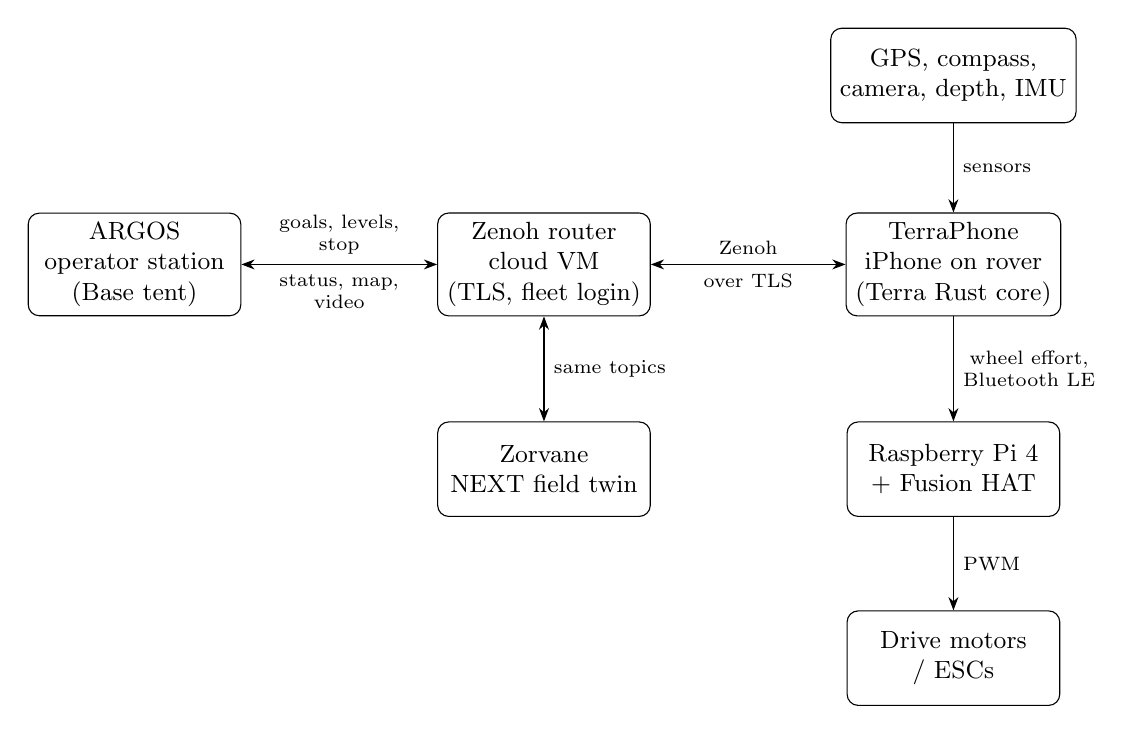
\begin{tikzpicture}[
  box/.style={draw, rounded corners, align=center, minimum width=2.7cm, minimum height=1.2cm, font=\small},
  lbl/.style={font=\scriptsize, align=center},
  >=Stealth]
  \node[box] (argos) at (0,0) {ARGOS\\operator station\\(Base tent)};
  \node[box] (router) at (5.2,0) {Zenoh router\\cloud VM\\(TLS, fleet login)};
  \node[box] (zorvane) at (5.2,-2.6) {Zorvane\\NEXT field twin};
  \node[box] (phone) at (10.4,0) {TerraPhone\\iPhone on rover\\(Terra Rust core)};
  \node[box] (pi) at (10.4,-2.6) {Raspberry Pi 4\\+ Fusion HAT};
  \node[box] (motors) at (10.4,-5.0) {Drive motors\\/ ESCs};
  \node[box] (gps) at (10.4,2.4) {GPS, compass,\\camera, depth, IMU};
  \draw[<->] (argos) -- node[lbl, above] {goals, levels,\\stop} node[lbl, below] {status, map,\\video} (router);
  \draw[<->] (router) -- node[lbl, above] {Zenoh} node[lbl, below] {over TLS} (phone);
  \draw[<->] (router) -- node[lbl, right] {same topics} (zorvane);
  \draw[->] (phone) -- node[lbl, right] {wheel effort,\\Bluetooth LE} (pi);
  \draw[->] (pi) -- node[lbl, right] {PWM} (motors);
  \draw[->] (gps) -- node[lbl, right] {sensors} (phone);
\end{tikzpicture}
\caption{The experimental environment. The operator station and the rover never talk directly: both connect out to one authenticated Zenoh router. Zorvane speaks the same topics as a real rover, so the operator station cannot tell them apart. Planning and control run on the phone; the Pi only applies wheel effort.}
\label{fig:env}
\end{figure}

\subsection{The router}
\label{sec:env-router}

All fleet traffic passes through one Zenoh router running on a small cloud virtual machine.
Zenoh is a publish--subscribe protocol \todo{cite Zenoh}; every rover, the ARGOS desktop application, and the Zorvane simulator connect \emph{out} to the router over TLS and authenticate with a fleet account.
All topics share one prefix, and each rover publishes and subscribes under its own numeric rover ID.
Because every party dials out, neither the operator's laptop nor the phone needs a public address or an open port, which is what lets a phone on a field connect to an operator in a tent without local network setup.
The same machine hosts an independent observability collector that stores timestamped diagnostic events from the phone, the operator station, and the simulator, and exports them for replay.

The router is not part of the control loop.
It carries intent (levels, goals, held teleoperation, stop) and telemetry (pose, status, occupancy, video signalling), but every motion decision is checked again on the vehicle.
Fleet membership allows publishing and subscribing; it does not give per-operator roles, and the vehicle's own runtime checks remain the final command boundary.
\todo{State whether the phone reaches the router over cellular data or over field Wi-Fi in the NEXT setup, and measure the round-trip latency from Field~3.}

\subsection{The phone as the brain}
\label{sec:env-phone}

An iPhone rides on the rover and runs TerraPhone, a Swift application around the shared Terra Rust core.
The phone provides every sensor the autonomy uses: the rear camera and ARKit visual--inertial pose, depth where the handset has it, the Core Motion IMU, GPS, and the compass.
The Rust core holds state estimation, a rolling local occupancy map (200~$\times$~200 cells at 0.1~m, so 20~$\times$~20~m), the control-authority arbiter, the planners, and velocity control.
The control loop ticks every 10~ms, and wheel commands go out every fifth tick, at 20~Hz.
The arbiter is the single owner of motion: teleoperation, assisted teleoperation, the two waypoint levels, exploration, target search, and task autonomy all pass through it, and an emergency stop latches until an explicit, healthy reset.

The phone does not run a second planner when it supervises the simulator; in that mode it sends goals and control intent to Zorvane instead.
Depthless handsets hold any level that needs a map.

\subsection{The Pi motor bridge}
\label{sec:env-pi}

The phone cannot drive motors directly, so a Raspberry Pi~4 with a SunFounder Fusion HAT acts as a motor bridge.
The phone sends normalized wheel effort to the Pi over Bluetooth Low Energy; the Pi applies it to motor ports or to PWM outputs for electronic speed controllers (ESCs).
The Pi runs no autonomy and none of the Rust crates.
It holds each drive command for 250~ms and then sets every output to its safe value, and an external battery cutoff removes motor power independently of both computers.
Zero effort coasts; it does not brake.
Section~\ref{sec:rover-electronics} describes how the Pi's own safety duties changed in October 2026.
Chapter~\ref{ch:rover} describes the hardware in detail, including the planned replacement of the Pi by a microcontroller attached to the phone over USB.

\subsection{The operator station}
\label{sec:env-argos}

The operator runs the ARGOS desktop application, written in Rust with the GPUI toolkit, on a laptop.
For NEXT the laptop sits in the alliance's Base, which is where the rules allow the team to be.
ARGOS shows each rover on one map over satellite imagery with its GPS fix and accuracy, a local occupancy map, first-person video over WebRTC, and the autonomy controls.
The operator selects Local or Outdoor GPS navigation and an autonomy level, sends goals by clicking the map, arms or disarms the hardware, and has stop and L0 manual control one click away.
ARGOS binds every non-neutral command to the rover's current run and authority revision, so a stale command from before a takeover or a reset is rejected by the vehicle rather than acted on.

Several changes in late October 2026 shaped how the operator works with it.
A goal is set with a single click on the map, which opens a confirm popup anchored to that point; nothing is sent until the operator presses Send goal, and a drag still pans the map.
The local occupancy grid is drawn on the main map under the rover, in the same frame as its goals, so a rover placed by GPS can also take local goals by a click on its grid; the separate local-map tab was removed.
When manual driving is refused, ARGOS names the failing check (no status yet, an unanswered command, stale status and its age, an active stop, a Terra hold with its reason, or a non-manual level) instead of one generic error.
The navigation panel shows the reported heading uncertainty and its age against the outdoor limits.
A Sim/Real toggle reconnects the whole dashboard to the simulator or to the real fleet at runtime, so one session can switch between Zorvane and a rover.
Capture~3D and Live~3D show the rover's labelled depth points, which is how the operator can see what the mapper thinks is ground and obstacle (Section~\ref{sec:auto-capture}).
A Task panel sends an L5 task and shows the model's plan, questions and recent steps (Section~\ref{sec:auto-l5}).
ARGOS has a user documentation site and downloadable builds for macOS, Windows and Linux, produced from a version tag; the first release is v0.1.0.

\subsection{Outdoor GPS navigation and heading}
\label{sec:env-gps}

On a 100~m field the phone's visual--inertial pose alone is not enough to reach a bucket on the other half: it drifts, and it has no notion of where the buckets are in the world.
Terra therefore has an outdoor GPS mode, in which a geographic goal (latitude and longitude) is converted, at most twice per second, into a local target up to 3~m ahead.
The local planner and the L3 footprint and braking checks still choose every command, and GPS never modifies the AR pose or the occupancy map.
Forward speed in this mode is capped at 0.3~m/s.

A mission is admitted only at L3, with armed hardware, fresh visual--inertial feedback, a healthy local map, a GPS fix no older than 3~s with accuracy of 10~m or better (and no worse than the arrival radius), and a heading no older than 2~s with accuracy of 30$^\circ$ or better.
The default arrival radius is 5~m, configurable from 2 to 20~m, and arrival is confirmed by three distinct fixes inside the radius.
Any loss of GPS, heading, tracking, map, arming, or authority latches a pause; recovery alone does not resume, and the operator must press Resume in ARGOS.
ARGOS independently holds an outdoor mission when the reported heading uncertainty exceeds $\pm$35$^\circ$.

Heading turned out to be the weak input.
The phone's magnetometer, mounted close to the drive motors, read headings with errors of 30--50$^\circ$, so a compass-only heading tripped the uncertainty hold often.
Since October 2026, Terra fuses three sources: the ARKit yaw carries the heading between corrections, the GPS course over ground (used only at 0.5~m/s or faster and while turning less than 10$^\circ$) gives a tight lock, and the compass only seeds the estimate and never claims to be better than its own reported accuracy.
In practice, the rover is driven in a straight line for a few seconds at the start of an outdoor run to lock its heading.
\todo{Measure heading error before and after the fusion on Field~3 and report it in the evaluation chapter.}

\subsection{Frontier exploration}
\label{sec:env-explore}

Searching a penalty box, or a sector of a disaster site, is a coverage task, and Terra implements it as time-bounded frontier exploration.
A frontier is a free map cell next to unknown space.
In the autonomous \texttt{explore} level, the rover repeatedly picks a frontier, scored by expected information gain, and drives to it through the same local planner and safety arbiter as every other level; there is no per-goal approval.
The run ends when its time budget expires, when no reachable frontier remains, when the operator stops or takes over, or when the map goes stale (older than 0.5~s) or a safety hold fires.
A blocked frontier is retried and, after three failures, excluded for the rest of the run.
Exploration reports elapsed and remaining time, the current target, and the observed free area, and logs each frontier choice.

In the ladder of Table~\ref{tab:intro-levels}, exploration and target search together make up L4: exploration covers ground, target search confirms objects in it.
ARGOS offers the two as separate controls, ``L4 Explore'' and ``Search''; both are reported as L4.
Above them, the L5 \texttt{task} level lets an on-phone language model choose waypoints for a task typed by the operator; it is implemented but has not yet run on a phone, and it is not part of the pilot study (Section~\ref{sec:auto-l5}).

\subsection{Zorvane: the NEXT field twin}
\label{sec:env-zorvane}

Zorvane is the project's simulator, built on the Bevy engine with Avian physics, and since October 2026 its only world is the NEXT field.
It places a 100~$\times$~64~m pitch on Field~3 at the field's mapped centroid and heading, taken from OpenStreetMap~\citep{osm2026field3}, with an ellipsoid height derived from USGS elevation and the NOAA GEOID18 offset.
Because of that placement, the simulator publishes a geographic localization report and simulated GPS on the same topics a real phone uses, so ARGOS shows the simulated rover on Field~3 and Terra's outdoor GPS navigation runs on the simulated field unchanged.
The surroundings (turf, fence, light towers, scoreboard, the two Base tents, and nearby buildings) are generated from OpenStreetMap footprints and given colliders.
Lighting can be set to noon, overcast, or evening for detector testing.

The game objects are modelled at regulation size: tennis balls of 6.70~cm diameter and 58~g, inside the ITF tolerances~\citep{itf2026rules}, and 5-gallon buckets from a product drawing (0.305~m top diameter, 0.340~m high), ten per half, four of them on 1~m stands, placed by a fixed random seed.
The default rover is CrabTrapBot, the team's NEXT robot (Chapter~\ref{ch:rover}).
A full scoring loop is implemented: the rover collects balls through its intake, returns to its own goal line, where collected balls become waiting, loads them one at a time into a two-ball dumper on operator command, parks with the outlet over a ground-level bucket of its alliance's colour, and dumps.
Balls fall under physics, and only balls that land in the bucket score, with the 1- and 2-point rule.
Launching, tagging, out-of-bounds penalties, and knocked-bucket penalties are explained in an intro cutscene but not enforced, so raised buckets are out of reach in simulation.

Earlier versions of Zorvane also held the reference disaster-search mission used to develop the autonomy levels, which was removed when the simulator became NEXT-only on October 24, 2026 (Chapter~\ref{ch:simulation}).

\subsection{Logging and measurement}
\label{sec:env-logging}

Every part of the environment records what it did.
Terra and Zorvane write a JSONL run log per run containing the mission definition, planner configuration, run identity, every control tick's output, authority requests and changes, mission progress, observed free area, contacts, and near-miss episodes (observed clearance below 0.3~m).
ARGOS exports operator session logs whose action tokens and teleoperation sequence numbers join to the rover's receipts, so one intervention is not counted twice.
An \texttt{experiment/status} topic pairs each rover's run clock with UTC, and clock offsets are kept rather than assumed away.
A trial is labelled as \emph{fixed} (one assigned level) or \emph{adaptive} (operator-chosen), and the assigned condition is recorded separately from the levels actually requested and in effect.
Truncated recordings are not counted as complete runs, and interaction counts are recorded as workload proxies, not as measured workload.

The phone also keeps an observability journal of sensor, estimator and controller samples, copied off the device after a session; its sample rate is configurable and defaults to 10~Hz.
For ground truth on motion, the environment can include an OptiTrack motion-capture system: a small bridge republishes its rigid-body pose on the fleet router, so the same laptop that drives the rover records both the rover's own pose and the true one on one clock (Chapter~\ref{ch:autonomy}).

\section{From the field to the real situation}
\label{sec:real-world}

NEXT is a game, and a soccer field is not a collapsed building.
The case for using it rests on a structural match: the problems the field forces on a team are the same problems the deployments in Chapter~\ref{ch:background} ran into, in a form that can be repeated and scored.
The ARGOS design notes describe the intended thesis experiment as ``real-world, NEXT-style search and rescue,'' with simulation used for algorithm development only.
Table~\ref{tab:next-mapping} lays out the correspondence.

\begin{table}[ht]
\centering
\small
\caption{How the NEXT environment maps to disaster response, and what each element lets the study measure.}
\label{tab:next-mapping}
\begin{tabularx}{\textwidth}{@{}>{\raggedright\arraybackslash}p{2.9cm} >{\raggedright\arraybackslash}X >{\raggedright\arraybackslash}X@{}}
\toprule
In NEXT & In a disaster response & What it tests here \\
\midrule
Base tent; vehicles may be touched only there & Command post at the edge of an unsafe zone; responders cannot walk into the hazard to fix a robot (SubT's single Human Supervisor) & Fully remote supervision; a stuck rover is lost until recovered remotely \\
Tennis balls spread in the penalty boxes & Victims, objects, or areas to be found and reported & Search and coverage (L4), detection, and confirmation by the operator \\
Buckets in the far half & Delivery or reporting points: casualty collection, supply drop, sensor placement & Long waypoint travel (L2--L3) and a precise final approach \\
Distance bonus near the opposing Base & Deeper, riskier targets are worth more & Trade-off between reward and the risk of travelling far from the operator \\
90-minute match & Time-critical response window & Mission success under a deadline; battery endurance \\
Tagged and frozen for 15 minutes & A robot disabled by debris, a fall, or a lost link & Fleet degradation and operator re-planning around a lost unit \\
$-7$ for a knocked bucket or a ball out of bounds & Collateral damage and unsafe actions & Safety cost of autonomy errors; when the operator chooses to take over \\
100~m outdoor field, GPS, a remote link & Large outdoor sites; phone GPS errors of up to 10~m at Surfside & GPS accuracy gates, heading fusion, and continuing an accepted mission through a link outage \\
Several robots per alliance, one Base & One operator, many robots & Fleet size per operator and attention scheduling \\
\bottomrule
\end{tabularx}
\end{table}

\subsection{The lessons from Chapter~\ref{ch:background}, on the field}

Each recurring lesson from real missions has a concrete counterpart in this environment.

\begin{itemize}
\item \textbf{Lost link (WTC 2001).}
  The wireless robot lost at the World Trade Center had no onboard autonomy to recover its link~\citep{murphy2004rescue}.
  In this environment the rover connects to a cloud router over a link that can drop.
  Terra's design keeps an accepted L3 waypoint mission running locally across a router outage, while expiring manual intent within its 500~ms lease and never re-arming or resuming on reconnection alone; simulated 120-second router outages were used to check this.
  On the field this can be tested by cutting the router link mid-mission.
\item \textbf{Simple control for responders (Fukushima 2011).}
  Quince had to be easy for first responders to drive~\citep{nagatani2011fukushima}.
  ARGOS keeps every level one click away, and the study is designed for operators who did not build the rover.
\item \textbf{One supervisor as the bottleneck (SubT 2021).}
  NEXT's Base rule recreates SubT's single-supervisor constraint~\citep{ackerman2021subtoperators} at a smaller scale.
  The ball-collection loop produces a steady stream of moments that need the operator, such as loading at the goal, approving a dump, freeing a stuck rover, which is the attention load the study measures.
\item \textbf{Shared picture and GPS error (Surfside 2021).}
  Drone teams at Surfside coordinated through a chat group and saw phone GPS errors of up to ten metres~\citep{murphy2021surfside}.
  ARGOS shows every rover on one map with its fix and accuracy, and Terra refuses outdoor missions when the fix is worse than 10~m.
\end{itemize}

\subsection{Where the analogy breaks}

The mapping has limits, and the thesis does not claim more than it supports.
The field is flat synthetic turf: there is no rubble, no stairs, no dust, and no confined space, so mobility and terrain are not tested.
A tennis ball is not a person: detecting an optic-yellow ball on green turf is far easier than finding a victim, and the simulator's survivor rule is not a sensor model.
The network fails because of distance and congestion, not because concrete blocks the radio, and the field has open sky for GPS that a building interior would not.
The opposing alliance is an adversary that a disaster site does not have, although tagging is a reasonable stand-in for losing robots to events outside the operator's control.
Finally, the competition rewards points, and a response rewards lives and information; the study therefore reports mission measures (success, time, interventions, time at each level) rather than treating the match score as the result.
\todo{Decide whether the study runs during the actual NEXT match, in practice sessions on Field~3 with the same rules, or both, and state which results come from which.}

\section{Study conditions on the NEXT field}
\label{sec:next-study}

The Introduction proposed a study with a \emph{fixed} condition, in which one autonomy level is locked for a run, and a \emph{free} condition, in which the operator switches levels at will and the system logs when, why, and in what context.
On the NEXT field, the deck's three mission types become concrete tasks: \emph{find a target} becomes locating balls or a specific bucket; \emph{scout a route} becomes reaching the far half; and \emph{cover a sector} becomes a time-bounded exploration of one penalty box.
The conditions the Introduction lists can each be produced on the field: communication loss by cutting the router link, fleet size by the number of rovers per operator, debris by placing extra obstacles, deadlines by the match clock or a shorter budget, and surprises by tagging or by moving a bucket.
The same tasks can be run first in Zorvane, against the same ARGOS interface, and then on Field~3.

\todo{Fix the task list, the number of rovers, the trial order and counterbalancing, the workload instrument, and ethics approval before running any human-subject trial.}
\todo{No trials have been run. Report results only in the evaluation chapter.}

\section{Summary}

The NEXT Competition 2026 gives this thesis a mission with fixed rules, a deadline, a large outdoor field, and a rule that confines the team to its Base.
The environment built for it connects an operator station and phone-brained rovers through one authenticated cloud router, keeps motion authority on the phone, drives the motors through a Pi bridge, navigates outdoors on GPS with a fused heading, explores frontiers autonomously, and has a simulated twin of the same field on the same topics.
The structure of a NEXT match maps onto the problems seen in real disaster response, communication loss, a single supervisor, too little or too much autonomy, and the need for one shared picture, while the field leaves out terrain and real victims.
The next chapter describes the rover that has to play it.

% Chapter 3: Physical design of the rover for NEXT. First draft.
% Sources: Zorvane VEHICLES.md, SCALE.md, simulator/NEXT.md,
%   crates/zorvane-vehicle/src/lib.rs, simulator/src/next_competition.rs;
%   Terra docs/hardware/*.md, crates/terra-actuators/presets/*.json,
%   docs/superpowers/specs/2026-10-06-bluetooth-actuator-layouts-design.md,
%   mobile/ios/README.md (phone mounting), docs/MOUNT_CALIBRATION_CHECKLIST.md,
%   docs/autonomy/turning-policy.md, docs/REAL_ROVER_TUNING.md; Terra issue #21;
%   "Project ARGOS - One Operator Many Robots" deck (Oct 23, 2026), slides 10, 18, 19, 22;
%   project notes on the RP2350 motor board (Oct 24, 2026).
% Dimensions come from CAD files read by the simulator, not from measurements of the
% built robot. Mass, battery, motor limits and the launcher are open and marked \todo.

\chapter{Rover Physical Design}
\label{ch:rover}

Chapter~\ref{ch:competition} described the NEXT field and the environment around the rover.
This chapter describes the rover itself: what the rules ask of its body, the two chassis the project uses, the ball-handling mechanism, the phone mount, the drive electronics, and the planned replacement of the motor bridge.
The guiding principle is the one from the Introduction: the phone is the robot's only computer, so the rest of the vehicle should be as simple and cheap as the task allows.

All dimensions below are taken from the CAD models as the Zorvane simulator reads them.
They describe the design, not the built robot, and Section~\ref{sec:rover-open} lists what still has to be measured.

\section{Design requirements from the rules}
\label{sec:rover-requirements}

Each rule in Table~\ref{tab:next-rules} turns into a physical requirement.

\begin{description}
\item[Ball handling.] The game object is a regulation tennis ball, about 6.7~cm in diameter and 58~g~\citep{itf2026rules}, and 99 of them start in each penalty box.
  The rover needs an intake that gathers balls from the turf without stopping for each one, a store to carry several, and a way to put them into a bucket.
\item[Bucket height.] A ground-level 5-gallon bucket has its rim about 0.34~m above the turf; a raised bucket's rim is about 1.34~m up.
  Dumping into a ground bucket needs an outlet above 0.34~m that can reach over the rim; scoring in a raised bucket needs a launcher.
\item[Knocked buckets cost seven points.] The front of the rover must be able to park against a bucket to dump without pushing it over or swallowing it into the intake.
\item[Distance and time.] The field is 100~m long and the match lasts 90 minutes.
  At the outdoor GPS mode's 0.3~m/s cap, a single crossing of the pitch takes about five and a half minutes, so drive speed, battery life, and traction on synthetic turf all matter.
\item[No touching outside the Base.] Every recovery from a fault has to be remote.
  The drive electronics must fail safe on their own, and the rover must not need a person to reset it after a lost link.
\item[Tagging.] A vehicle hit by a launched ball is frozen for 15 minutes.
  The body cannot prevent this, but a smaller profile is a smaller target.
\end{description}

\section{Two chassis}
\label{sec:rover-chassis}

The project uses two bodies with the same software.
Both are differential-drive vehicles, so Terra's controllers, planners, and arbiter run on either; only the geometry, the wheel layout, and the actuator mapping change.
Table~\ref{tab:rover-bodies} compares them.

\begin{table}[ht]
\centering
\caption{The two rover bodies, from their CAD models as used by the simulator. \todo{replace with measured values from the built robots}}
\label{tab:rover-bodies}
\begin{tabularx}{\textwidth}{@{}l X X@{}}
\toprule
 & Terra development chassis & CrabTrapBot (NEXT rover) \\
\midrule
Role & Development and indoor obstacle-avoidance tests & Competition robot for NEXT \\
Size (W~$\times$~H~$\times$~L) & 0.403~$\times$~0.144~$\times$~0.384~m & 0.607~$\times$~0.614~$\times$~0.601~m \\
Wheels & Four, radius 45~mm & Four goBILDA 144~mm wheels (radius 72~mm) \\
Track width & 0.350~m & 0.526~m between tyre centres \\
Wheelbase & 0.240~m & \todo{measure} \\
Steering & Differential, skid-steer & Differential, four-wheel skid-steer \\
Motor outputs & Four DC motors on Fusion HAT motor ports (\texttt{terra-mini} layout) & ESCs on Fusion HAT servo (PWM) pins \\
Ball handling & None & Intake, internal store, top dumper \\
Phone mount & Portrait, top edge up, rear camera forward & Landscape, rear camera forward \\
Mass & \todo{measure; simulator uses 20~kg} & \todo{measure; simulator uses 20~kg} \\
\bottomrule
\end{tabularx}
\end{table}

\subsection{The Terra development chassis}

The development chassis is the small rover used for the indoor L3 obstacle-avoidance demonstrations in the Introduction.
Its CAD model is published in centimetres; reading those units as inches had once made the simulated rover 2.54 times too large, and the model is now scaled from its own unit metadata.
Its four DC motors connect to the Fusion HAT motor ports, two per side, and the committed \texttt{terra-mini} layout routes left effort to ports M2 and M3 and right effort to M0 and M1, each limited to $\pm$0.4 effort and half power until the drive is calibrated.

\subsection{CrabTrapBot}

CrabTrapBot is the team's NEXT robot, designed in Fusion and modelled in the simulator from its STEP export.
It is a roughly 0.6~m cube on four goBILDA 144~mm wheels, with a low, open-front intake and a dumper on top.
Its four wheels skid-steer, so the rover turns by dragging its wheels sideways, and its effective turning track on turf is wider than the 0.526~m geometric track.
Its propulsion is driven through ESCs on the Fusion HAT's PWM pins rather than through the HAT's motor ports.
NEXT robots have historically combined an intake with a shooter for balls (Terra issue \#21); CrabTrapBot's design as modelled has the intake and a gravity dumper, and no launcher.
\todo{Describe the built robot: frame material, motors and gearboxes, ESC model, and whether a launcher is planned for raised buckets.}

\section{Ball handling}
\label{sec:rover-balls}

CrabTrapBot's name describes its intake.
Balls enter through a low opening across the front, past inward-swinging flaps that let a ball in but not back out, like the funnel of a crab trap.
Inside, balls collect in a holding area.
In the simulator the store holds up to eight balls; when it is full the flaps stay shut and a front bar closes the chassis, so further balls stay on the field rather than jamming the intake.
\todo{Confirm the real store capacity and the flap mechanism (sprung or gravity).}

An upper front guard sits above the intake opening, at a height that lets balls pass underneath while keeping a bucket outside the chassis.
This is the design answer to the seven-point knocked-bucket penalty: the rover can drive its front against a bucket to dump without the bucket entering the intake.

Delivery uses a top-mounted dumper.
At the rover's own goal line, collected balls are moved, one per operator command, from the store into the dumper, which holds two balls about 0.6~m above the turf with its outlet just beyond the front of the chassis.
The rover then drives into the opponent's half, parks against a ground-level bucket, and dumps when the outlet is within 9~cm of the bucket opening.
A 0.6~m outlet clears the 0.34~m rim of a ground bucket but not the 1.34~m rim of a raised one, so raised buckets, worth three or six points, need a launcher that the current design does not have.
In the simulator the dump chute is idealized; panel geometry, hinge torque, and ball contact with the panels are not modelled.
\todo{Measure the real dumper's outlet height and the success rate of a dump into a ground bucket.}

The load-at-goal step is deliberately an operator action.
It gives the operator a defined, repeatable moment of attention per scoring cycle, which is useful for the study: it is a natural place to measure how quickly an operator responds when several rovers reach their goal lines at once.

\section{The phone mount}
\label{sec:rover-mount}

The phone is the rover's only sensor head, so its mount sets what the rover sees.
On both chassis the rear camera faces forward.
On the development chassis the phone stands upright in portrait with its screen facing backward; on CrabTrapBot it is mounted in landscape, rolled $\pm$90$^\circ$, and the roll is entered in the app's mounting settings.
The software keeps separate transforms from the phone's motion axes and from ARKit's camera axes to the rover body, and the compass reference follows whichever phone edge is most horizontal in the saved mount.

A mount calibration procedure records the camera height above the ground and any roll, pitch, and yaw relative to the rover axes, then fits the camera's forward and left offsets from two slow in-place turn passes with the motors disabled.
The mount must be rigid: any play between phone and chassis appears as pose error.
\todo{Report the measured camera height and offsets for CrabTrapBot.}

The mount's position also affects the compass.
Close to the drive motors, the phone's magnetometer read headings with errors of 30--50$^\circ$, which is why Terra fuses visual--inertial yaw, GPS course, and the compass rather than trusting the compass (Section~\ref{sec:env-gps}).
Moving the phone further from the motors is a physical mitigation worth testing alongside the software one.
\todo{Test heading error at two or more mount heights on CrabTrapBot.}

\section{Drive electronics}
\label{sec:rover-electronics}

\subsection{The Pi motor bridge}

Today the phone drives the motors through a Raspberry Pi~4 with a SunFounder Fusion HAT.
The phone sends normalized actuator commands over Bluetooth Low Energy; the Pi validates them and writes them to the HAT.
The Pi software is a single compiled ARM64 executable, so no Python installation or source checkout is needed on the rover.
A configurable layout of up to 16 actuators maps commands to outputs of four kinds: DC motors (signed effort), bidirectional ESCs (reverse, neutral, and forward pulse widths), unidirectional ESCs, and positional servos.
ESC and servo outputs use 50~Hz pulses, and the DC motor channels use a separate 100~Hz timer group so that the two do not share a timer.

\subsection{Safety in the hardware path}

Because nobody may touch the rover outside the Base, the hardware path must fail safe on its own.
The Pi enforces, independently of the phone:

\begin{itemize}
\item an explicit arm step; connecting or pairing never arms the motors;
\item a 200~ms command watchdog, after which outputs go to their safe state;
\item a safe state per output kind: zero power for DC motors, a continuous neutral or stop pulse for ESCs (never a zero-width pulse, which some ESCs read as a fault), and a configured safe position for servos;
\item an external battery cutoff switch that removes motor power and that the Pi cannot override.
\end{itemize}

Zero effort coasts rather than brakes.
The Raspberry Pi image used on the rover adds a fallback Wi-Fi hotspot and SSH over the USB-C port, so a technician at the Base can reach the Pi without the field network.

\subsection{Skid-steer turning}

A four-wheel skid-steer rover scrubs its tyres whenever it turns, and turning in place on turf is hard on the drivetrain and on the phone's pose estimate.
Terra applies a shared turning policy to all managed commands (ARGOS teleoperation and every autonomous level): yaw rate is limited to 0.5~rad/s, turns ramp in and out, the minimum turning radius is 0.5~m, turning in place is off by default, and reverse is limited to 0.15~m/s.
These are software starting values, not calibrated limits.
\todo{Calibrate the turning limits on CrabTrapBot on synthetic turf.}

\section{Power}
\label{sec:rover-power}

The rover carries two energy stores: its drive battery, which also powers the Pi, and the phone's own battery.
A 90-minute match sets the endurance target for both.
TerraPhone keeps the screen awake while its scene is active, and continuous camera, depth, GPS, and network use draw the phone battery quickly.
\todo{Specify the drive battery (chemistry, voltage, capacity) and measure drive and phone endurance over a 90-minute run on turf.}

\section{Planned: a USB microcontroller in place of the Pi}
\label{sec:rover-rp2350}

The Pi is the last general-purpose computer on the rover, and the phone-as-brain argument says it should go.
It costs money, needs an operating system image to flash and maintain, boots slowly, and adds a Bluetooth link that can drop.
The long-term plan is a cheap microcontroller attached to the phone as a USB peripheral.

The chosen part is an RP2350 that enumerates as a USB network device (a CDC-NCM or CDC-ECM Ethernet gadget) on the iPhone's USB-C port.
The phone would then send wheel commands over that wired network link, which avoids the accessory certification that iOS requires for a raw USB serial device.
The microcontroller would keep the Pi's safety duties: arming, a watchdog, and safe output states.

Two risks come first.
The phone-side risk is whether iOS brings up a generic USB network link from such a device at all; this has not been bench-tested.
The network-side risk is that the board must not advertise a default route or a DNS server, or the phone might send its router traffic over the USB link and lose its connection to ARGOS.
\todo{Bench-test the RP2350 USB network link on the rover's iPhone before committing the design; report the result here.}

\section{Open measurements}
\label{sec:rover-open}

Several numbers in this chapter are still design values or simulator placeholders.
Before any of them appear in results, they must be measured on the built robot:
mass (the simulator uses 20~kg, unsourced), motor and ESC limits and the resulting top speed (the simulator keeps a 2.29~m/s cap carried over from an earlier model), wheelbase, store capacity, dumper outlet height, phone mount offsets, battery specification and endurance, and the turning limits on turf.
\todo{Add a photo and a labelled drawing of CrabTrapBot.}
\todo{Add a bill of materials with costs, to support the low-cost argument.}

% Chapter 4: Simulation (Zorvane). First draft.
% Sources: Zorvane repository at 3ddfc92 (Oct 24, 2026): README.md, SCALE.md, VEHICLES.md,
%   simulator/NEXT.md, simulator/DEPTH_CAMERA.md, docs/src/pages/*.md, Cargo.toml,
%   terra-source.json, simulator/src/*.rs module headers and defaults
%   (depth_camera.rs, velocity_controller.rs, physics.rs, terra.rs, outdoor.rs,
%   control_queue.rs, fpv/, bridge_recording.rs), and commit 5481b47 (NEXT-only);
%   Terra docs/autonomy/README.md; ARGOS docs/design/3d-dashboard.md.
% Numbers are simulator defaults read from the code, not measurements.
% Citations for Bevy, Avian, Gazebo and AirSim are from general knowledge: VERIFY.

\chapter{Simulation}
\label{ch:simulation}

Chapter~\ref{ch:competition} introduced Zorvane as the digital twin of the NEXT field.
This chapter describes the simulator itself: what it is for, how it is built, what it models and what it leaves out, and how it is used in this thesis.
The guiding rule is that the simulator must be indistinguishable from a real rover \emph{at the interface}: an operator station or a test script connected to Zorvane should not need to know that no hardware exists.
Below that interface, the simulator is deliberately simpler than the world, and Section~\ref{sec:sim-fidelity} lists exactly where.

\section{Role in the thesis}
\label{sec:sim-role}

The simulator has four jobs.

\begin{enumerate}
\item \textbf{Algorithm development.}
  The autonomy levels, from assisted teleoperation to frontier exploration, were developed against the simulator before they were run on a phone.
  Because Zorvane links the same Terra crates the phone uses, a change to a planner is exercised in simulation with no porting step.
\item \textbf{Interface development.}
  ARGOS was built and tested against Zorvane: the fleet map, autonomy controls, waypoint goals, held teleoperation, first-person video, and outdoor GPS missions all work against the simulator before they meet a rover.
\item \textbf{Scale.}
  A team owns a handful of rovers; the simulator can field up to 32.
  The ARGOS design notes plan to repeat the study measures at 15 to 20 vehicles, a fleet size that is only practical in simulation.
\item \textbf{Practice and training.}
  The NEXT field, its rules, and its scoring loop let a team rehearse a match, and let a study participant learn the operator station, before going to Field~3.
\end{enumerate}

The simulator is \emph{not} the venue for the thesis's main results.
The ARGOS design notes state that the thesis experiment is real-world, NEXT-style search and rescue, and that the simulator is for algorithm development.
Results obtained in Zorvane are reported as such and are not presented as evidence of physical performance.

\section{Why a custom simulator}
\label{sec:sim-why}

General robotics simulators such as Gazebo~\citep{koenig2004gazebo} and photorealistic ones such as AirSim~\citep{shah2017airsim} are the usual choices for ground robots.
Zorvane was written instead, in Rust, for three reasons that follow from the rest of the system.
First, Terra's autonomy is a Rust library; a Rust simulator links it directly, with no middleware bridge and no second implementation to keep in step.
Second, the operator contract is Zenoh topics with specific JSON payloads, run and authority revisions, and WebRTC video; matching that contract exactly was simpler in a simulator built around it than by adapting a general one.
Third, the NEXT field is a specific, flat, outdoor place, which needs accurate geography and game logic more than it needs articulated-body dynamics or terrain.
\todo{Add a short comparison with ROS~2 and Gazebo-based fleet simulators, and say what Zorvane gives up by not using them.}

\section{Architecture}
\label{sec:sim-arch}

Zorvane is built on the Bevy game engine~\citep{bevy2026} with the Avian physics engine~\citep{avian2026}.
One Bevy unit is one metre.
The repository is a Rust workspace with two members: the simulator binary and a vehicle-body crate.
The robotics crates (types, control, waypoint following, mapping, navigation, state estimation, transport, autonomy, and the experiment recorder) stay in the Terra repository, where the phone also compiles them, and Zorvane builds against a pinned Terra revision recorded in the repository.
Pinning keeps the phone and the simulator on the same autonomy code, and makes every simulated run traceable to an exact revision.

Figure~\ref{fig:sim-arch} shows the main parts.

\begin{figure}[ht]
\centering
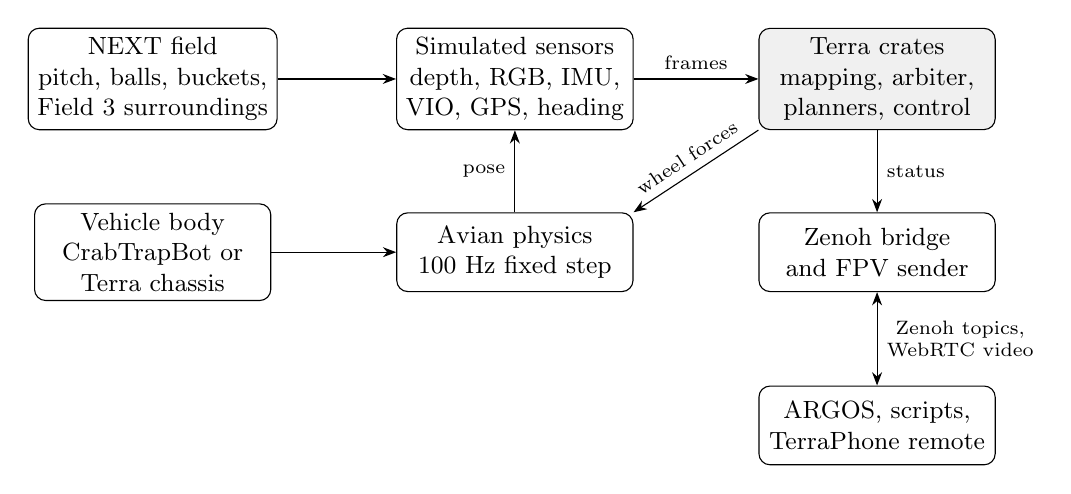
\begin{tikzpicture}[
  box/.style={draw, rounded corners, align=center, minimum width=3.0cm, minimum height=1.0cm, font=\small},
  terra/.style={box, fill=black!6},
  lbl/.style={font=\scriptsize, align=center},
  >=Stealth]
  \node[box] (world) at (0,0) {NEXT field\\pitch, balls, buckets,\\Field~3 surroundings};
  \node[box] (body) at (0,-2.2) {Vehicle body\\CrabTrapBot or\\Terra chassis};
  \node[box] (sensors) at (4.6,0) {Simulated sensors\\depth, RGB, IMU,\\VIO, GPS, heading};
  \node[box] (physics) at (4.6,-2.2) {Avian physics\\100~Hz fixed step};
  \node[terra] (terra) at (9.2,0) {Terra crates\\mapping, arbiter,\\planners, control};
  \node[box] (bridge) at (9.2,-2.2) {Zenoh bridge\\and FPV sender};
  \node[box] (out) at (9.2,-4.4) {ARGOS, scripts,\\TerraPhone remote};
  \draw[->] (world) -- (sensors);
  \draw[->] (body) -- (physics);
  \draw[->] (sensors) -- node[lbl, above] {frames} (terra);
  \draw[->] (terra) -- node[lbl, right] {status} (bridge);
  \draw[->] (terra.south west) -- node[lbl, above, sloped] {wheel forces} (physics.north east);
  \draw[->] (physics) -- node[lbl, left] {pose} (sensors);
  \draw[<->] (bridge) -- node[lbl, right] {Zenoh topics,\\WebRTC video} (out);
\end{tikzpicture}
\caption{Zorvane's structure. The shaded box is Terra's own code, linked unchanged. Everything a client sees passes through the bridge, on the same topics a real rover uses.}
\label{fig:sim-arch}
\end{figure}

\subsection{Vehicle bodies}

A vehicle is a plug-in: a body declares its identifier, its visual model, its chassis box and mass, and its locomotion.
Two bodies are registered: CrabTrapBot, the default NEXT rover, and the Terra development chassis (Chapter~\ref{ch:rover}).
Both are differential drive; the simulator turns a differential-drive body into a wheel controller and a physics configuration, and refuses at startup to drive a body whose locomotion it does not support.
That refusal is the extension point for other vehicle types, such as a drone, without forking the world or the topic layout.

\subsection{Physics and drive}

Each rover is a single dynamic rigid body, a box the size of the chassis, with yaw free and roll and pitch locked.
Wheel commands become forces on that body, with linear, lateral, and yaw drag tuned so that the rover accelerates, coasts, and resists sideslip plausibly.
Physics and control run on a 100~Hz fixed step.
Wheel odometry is ideal.
There are no wheel joints, no tyre model, and no suspension; skid-steer scrub, for example, is represented only through drag.

\subsection{Sensors}

Each rover carries a front-mounted depth sensor and a colocated RGB camera, both rendered on the GPU and read back asynchronously.
The default depth sensor is 256~$\times$~192 pixels with a 60$^\circ$ vertical field of view and a range of 0.05 to 30~m, and reports axial depth in metres with NaN for no return.
It is an ideal sensor: it has no noise and no housing, and it sees opaque and alpha-masked geometry, including meshes with no collider.
Depth frames carry the camera and body pose at exposure time, so the rover's occupancy map is built from exposure-aligned frames exactly as on the phone.

The velocity controller receives phone-like feedback, an IMU sample every physics step and a visual--inertial pose at 20~Hz, taken from the simulated body.
Because the Field~3 placement gives the pitch a geographic origin and heading, the simulator also produces GPS fixes and a true heading from the rover's pose.
These are exact: they are sampled from ground truth and reported with an accuracy of 1~m and 1$^\circ$.
Section~\ref{sec:sim-fidelity} returns to what that means for outdoor results.

\subsection{The bridge}

The bridge is the simulator's only external interface.
It publishes and subscribes on the same Zenoh topics as TerraPhone, under a configurable prefix, so a client can be pointed at Zorvane, at a real rover, or at the cloud router without changes.
It applies the same command rules the phone applies.
Every non-neutral command must carry the current run identifier and authority revision.
A teleoperation command expires after 500~ms.
A stop dominates every other request received in the same control tick, including a reset, and a full command queue drops the oldest non-stop request first.
Messages larger than 2048 bytes are ignored.

Telemetry rates match the phone's defaults: pose and camera frames at up to 10~Hz, status topics at about 5~Hz, and occupancy as full snapshots when the map changes, or at least every two seconds, with lightweight heartbeats in between.
First-person video is H.264 over WebRTC, using the same signalling as TerraPhone, and the camera renders only while a call is live.
A rover can be armed and disarmed, and the simulated actuator relay reports readiness like the real Pi bridge.

\subsection{Game logic}

The NEXT rules in Section~\ref{sec:next-rules} are implemented as simulator systems: the intake that captures balls entering CrabTrapBot's opening, the store and its capacity, the waiting state at the goal line, operator-triggered loading into the dumper, the dump readiness check, ball physics into the bucket, and the score.
The two game actions, load and dump, are also Zenoh topics, and \texttt{next/status} reports each rover's stage (searching, carrying balls, full and returning, or waiting for the operator), so the game loop can be driven and observed from ARGOS or a script.

\section{Running the simulator}
\label{sec:sim-running}

Zorvane runs as a desktop application with a start menu, in which the user picks the number of rovers, followed by a narrated cutscene of the rules.
It also runs headless, with no window, for automated checks.
Release builds for macOS, Windows, and Linux are produced by continuous integration from a version tag, so an operator or study participant can run the simulator without a Rust toolchain; the first tag is v0.1.0, from October 24, 2026.
Environment variables select the rover count, the topic prefix and listener, the bucket seed, the lighting, extra balls, the camera view, and whether video is on.

For a study session the simulator can connect to the same authenticated cloud router as the real fleet, under its own prefix, so that the operator station is configured once.
\todo{Describe the exact session setup for simulated trials: local listener or cloud router, rover count, seed list.}

\subsection{An AI model as a player}
\label{sec:sim-mcp}

Zorvane can also be played by a language model instead of a person (Zorvane PR~\#26, open and unmerged at the time of writing).
A small server exposes one rover through the Model Context Protocol (MCP), so any MCP client can call it as a set of tools: read the match state and score, look through the forward camera as an image, read the occupancy map as text, choose an autonomy level from L0 to L4, send a waypoint goal at L2 or L3, drive a teleoperation burst of at most 5~s at up to 2~m/s, stop, and press the NEXT load and dump buttons.
Bucket positions are not exposed, so the model has to find buckets by looking.
The server uses the same Zenoh topics and the same run and authority binding as ARGOS, so the model's commands pass the rover's checks exactly as an operator's do.
In a headless test run, a model client read the match state, took a camera image, drove, changed level, and reached an L2 goal; L3 goals and the text map were not verified, because the software-rendered run published no occupancy map, and loading and dumping were not exercised.

This differs from L5 (Section~\ref{sec:auto-l5}).
In L5 the model runs on the phone and only proposes waypoints to the arbiter; here the model runs off-board and plays the role of the operator, including the choice of autonomy level.
That makes it a way to study level choice itself: a model, or a learned policy, can choose the level for each phase of a match, and its choices can be compared with an operator's.
\todo{Merge the MCP server, verify L3 goals and the map on a GPU machine, and decide whether model-played matches become part of the evaluation.}

\section{Logging and repeatability}
\label{sec:sim-logging}

Every simulated run writes the same JSONL run log as the phone, through Terra's run recorder: the run identity and configuration, each control tick's output, authority events, mission progress, observed free area, contacts, and near misses.
The simulator also sends diagnostic events to the observability collector described in Chapter~\ref{ch:competition}.

Repeatability comes from three things: the pinned Terra revision, a fixed seed for the bucket layout (and for any extra balls), and a fixed rover spawn on the goal lines.
Rendering and physics run on the host's GPU and CPU, so two runs with the same seed are not guaranteed to be bit-identical, but they start from the same state and follow the same rules.
\todo{Measure run-to-run variation for a fixed scripted mission, to state how repeatable a simulated trial is.}

The test suite runs without a graphics device; tests that need a real GPU, such as checking a rendered wall distance in metres, are marked to run only on request.

\section{Fidelity and the reality gap}
\label{sec:sim-fidelity}

Table~\ref{tab:sim-fidelity} lists what Zorvane models and what it simplifies or omits, and what each gap means for the thesis.

\begin{table}[ht]
\centering
\small
\caption{Simulator fidelity, from the simulator's own code and documentation.}
\label{tab:sim-fidelity}
\begin{tabularx}{\textwidth}{@{}>{\raggedright\arraybackslash}p{2.6cm} >{\raggedright\arraybackslash}X >{\raggedright\arraybackslash}X@{}}
\toprule
Aspect & In Zorvane & Consequence \\
\midrule
Interface & Same topics, payloads, command rules, rates, and video signalling as TerraPhone & Operator-facing behaviour transfers directly; this is what the simulator is built to get right \\
Autonomy code & Terra crates linked unchanged at a pinned revision & Planner and arbiter logic is the same; its inputs are not \\
Field & 100~$\times$~64~m pitch at Field~3's geographic placement; OpenStreetMap surroundings; flat & Distances, layout, and GPS frame match; terrain does not \\
Depth & Ideal GPU depth, 256~$\times$~192, no noise & Obstacle avoidance looks better than on a phone with noisy or missing depth \\
Pose & IMU and VIO from ground truth; ideal odometry & No VIO drift or tracking loss \\
GPS and heading & Exact, reported at 1~m and 1$^\circ$ & The GPS accuracy gate and the heading problem (Section~\ref{sec:env-gps}) never trigger; outdoor results must come from Field~3 \\
Physics & One rigid box, roll and pitch locked, drag-based skid & No tyre slip, tipping, or turf effects; turning limits must be calibrated on the real rover \\
Mass and motor limit & 20~kg and a 2.29~m/s cap, both unsourced placeholders & Speeds and accelerations are indicative only \\
Ball handling & Idealized intake and dump chute & Scoring in simulation is an upper bound on the real mechanism \\
Rules & Scoring for ground buckets only; launching, tagging, and penalties not enforced & Simulated matches are practice, not full matches \\
Network & Local or router link; no injected loss & Communication loss must be added deliberately for a study \\
\bottomrule
\end{tabularx}
\end{table}

The pattern is consistent: Zorvane is faithful where the operator meets the system, and idealized where the robot meets the world.
That suits the thesis's question, which is about how an operator supervises robots at different levels of autonomy, more than about how well any one robot perceives.
It also sets a clear rule for reporting.
Interface-level measures from the simulator, such as how often an operator switches level, how quickly they respond, and how many interventions a mission takes, are meaningful as practice and pilot data.
Robot-level measures, such as obstacle clearance, navigation success, and GPS arrival accuracy, are reported only from the real rover.
\todo{Add sensor noise, VIO drift, GPS error, and link loss as configurable options, and report which were enabled for any simulated result.}

\section{History}
\label{sec:sim-history}

The simulator began inside the Terra repository as a Bevy world for developing the rover's control and autonomy, and was moved into its own repository, Zorvane, with the shared robotics crates left in Terra.
Over October 2026 it held several worlds: a practice town, real elevation tiles around George Mason University, photorealistic 3D-tile scenery, a seeded disaster-search mission with broken walls, rubble, and three hidden simulated survivors, and a browser build.
On October 24, 2026, Zorvane was reduced to the single NEXT field; the other worlds, the survivor mission and its detector, and the browser build were removed.
Terra's documentation still describes the disaster-search mission, and its mission bookkeeping remains in the shared code, which ARGOS still reads.
\todo{Decide whether the disaster-search mission is needed for the study; if so, restore it from history at a pinned revision and describe it here.}

\section{Summary}

Zorvane is a Rust simulator of the NEXT field that links Terra's autonomy unchanged and speaks exactly the protocol a real rover speaks.
It supports algorithm and interface development, fleets larger than the team can build, and practice on the competition field.
Its sensors, pose, GPS, and physics are idealized, so it is used for operator-facing measures and pilot work, and every robot-level claim in this thesis is checked on the real rover.
The next chapter describes the software architecture and the autonomy levels that run in both places.


\bibliographystyle{plainnat}
\bibliography{references}

\end{document}
